% --------------------------------------------------------------
% This is all preamble stuff that you don't have to worry about.
% Head down to where it says "Start here"
% --------------------------------------------------------------
 
\documentclass[12pt]{article}
 
\usepackage[margin=1in]{geometry} 
\usepackage{amsmath,amsthm,amssymb}
\usepackage{mathtools}
\usepackage{multicol}
\usepackage{textcomp}
\usepackage{float}
\usepackage{longtable}
\usepackage{hyperref}
 
\newcommand{\N}{\mathbb{N}}
\newcommand{\Z}{\mathbb{Z}}
\newcommand\aug{\fboxsep=-\fboxrule\!\!\!\fbox{\strut}\!\!\!}
 
\newenvironment{theorem}[2][Theorem]{\begin{trivlist}
\item[\hskip \labelsep {\bfseries #1}\hskip \labelsep {\bfseries #2.}]}{\end{trivlist}}
\newenvironment{lemma}[2][Lemma]{\begin{trivlist}
\item[\hskip \labelsep {\bfseries #1}\hskip \labelsep {\bfseries #2.}]}{\end{trivlist}}
\newenvironment{exercise}[2][Exercise]{\begin{trivlist}
\item[\hskip \labelsep {\bfseries #1}\hskip \labelsep {\bfseries #2.}]}{\end{trivlist}}
\newenvironment{reflection}[2][Reflection]{\begin{trivlist}
\item[\hskip \labelsep {\bfseries #1}\hskip \labelsep {\bfseries #2.}]}{\end{trivlist}}
\newenvironment{proposition}[2][Proposition]{\begin{trivlist}
\item[\hskip \labelsep {\bfseries #1}\hskip \labelsep {\bfseries #2.}]}{\end{trivlist}}
\newenvironment{corollary}[2][Corollary]{\begin{trivlist}
\item[\hskip \labelsep {\bfseries #1}\hskip \labelsep {\bfseries #2.}]}{\end{trivlist}}
 
\begin{document}
 
% --------------------------------------------------------------
%                         Start here
% --------------------------------------------------------------
 
%\renewcommand{\qedsymbol}{\filledbox}
 

% --------------------------------------------------------------
%     You don't have to mess with anything below this line.
% --------------------------------------------------------------
% --------------------------------------------------------------
% This is all preamble stuff that you don't have to worry about.
% Head down to where it says "Start here"
% --------------------------------------------------------------
 

% --------------------------------------------------------------
%                         Start here
% --------------------------------------------------------------
 
%\renewcommand{\qedsymbol}{\filledbox}

\title{TUTORIAL 10 - More recaps}%replace X with the appropriate number
\author{TRISTAN GLATARD\\ %replace with your name
COMP 361 Numerial Methods} %if necessary, replace with your course title
\date{November 23, 2018} 
\maketitle

\begin{exercise}{1} %You can use theorem, proposition, exercise, or reflection here. 

\begin{figure}[h]
    \centering
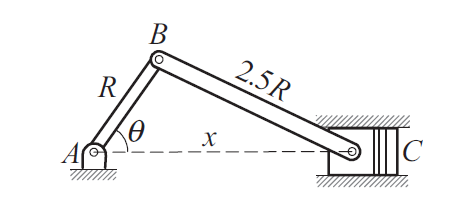
\includegraphics{5-1-12.png}
\end{figure}

The crank AB of length R = 90 mm is rotating at a constant angular speed of $d\theta/dt = 5 000$ rev/min. The position of the piston C can be shown to vary with
the angle $\theta$ as
$$x=R(cos\theta + \sqrt{2.5^2-sin^2\theta})$$
Use numerical differentiation to compute the acceleration at $\theta=0^0, 5^0, 10^0$

\textbf{Solution.} 
The acceleration is the second derivative of $x = f(\theta)= R(cos\theta + \sqrt{2.5^2-sin^2\theta})$. We will use central different approximation to calculate the acceleration at $\theta=0^0, 5^0, 10^0$ with $h=0.1$ (radian!) and $R = 0.09$ m. In this case, the approximation has the form:
$$f^{\prime\prime}(\theta) \approx \frac{f(\theta-h) -2f(\theta) + f(\theta+h)}{h^2}$$
Calculations are on the following table, note that we need to convert $\theta$ from degree to radian.

\begin{table}[h]
\centering
\begin{tabular}{|rrrrrr|}
\hline
\multicolumn{1}{|c}{\textbf{$\theta$(deg)}} & \multicolumn{1}{c}{\textbf{$\theta$(rad)}} & \multicolumn{1}{c}{\textbf{$f(\theta-h)$}} & \multicolumn{1}{c}{\textbf{$f(\theta)$}} & \multicolumn{1}{c}{\textbf{$f(\theta+h)$}} & \multicolumn{1}{c|}{\textbf{$f^{\prime\prime}(\theta)$}} \\ \hline
0 & 0.0000 & 0.3144 & 0.3150 & 0.3144 & -0.1258 \\
5 & 0.0873 & 0.3150 & 0.3145 & 0.3128 & -0.1250 \\
10 & 0.1745 & 0.3147 & 0.3131 & 0.3103 & -0.1225 \\ \hline
\end{tabular}
\end{table}

\end{exercise}

%EXERCISE 2-----------------------------------------------------
\begin{exercise}{2} %You can use theorem, proposition, exercise, or reflection here.  

The following table shows the power P supplied to the driving wheels of a car as a
function of the speed v. If the mass of the car is m = 2000 kg, determine the time
$\Delta t$ it takes for the car to accelerate from 1 m/s to 6 m/s. Use the trapezoidal rule
for integration. Hint: 	$\Delta t = m \int_{1s}^{6s}(v/P)dv$ , which can be derived from Newton’s
law $F = m(dv/dt)$ and the definition of power $P = Fv$.

\begin{table}[h]
\centering
\begin{tabular}{|c|c|c|c|c|c|c|c|c|c|c|c|}
\hline
v (m/s) & 0& 1.0& 1.8& 2.4& 3.5& 4.4& 5.1& 6.0\\ \hline
P (kW) &0 &4.7& 12.2 &19.0& 31.8& 40.1& 43.8 &43.2 \\ \hline
\end{tabular}
\end{table}

\textbf{Solution.}


Let f(v) = v/P, we transform the given table into 
\begin{table}[h]
\centering
\begin{tabular}{|c|c|c|c|c|c|c|c|c|c|c|c|}
\hline
v (m/s) & 0& 1.0& 1.8& 2.4& 3.5& 4.4& 5.1& 6.0\\ \hline
$f(v)*10^{-3}$ &0 &0.2128&	0.1475&	0.1263&	0.1101	&0.1097&0.1164	&0.1389
 \\ \hline
\end{tabular}
\end{table}

Apply trapezoidal rule on each panel,

\begin{table}[h]
\centering
\begin{tabular}{|rrrrrr|}
\hline
\multicolumn{1}{|c}{\textbf{a}} & \multicolumn{1}{c}{\textbf{b}} & \multicolumn{1}{c}{\textbf{h}} & \multicolumn{1}{c}{\textbf{$f(a)*10^{-3}$}} & \multicolumn{1}{c}{\textbf{$f(b)*10^{-3}$}} & \multicolumn{1}{c|}{\textbf{$I*10^{-3}$}} \\ \hline
1 & 1.8 & 0.8 & 0.2128 & 0.1475 & 0.14412 \\
1.8 & 2.4 & 0.6 & 0.1475 & 0.1263 & 0.08214 \\
2.4 & 3.5 & 1.1 & 0.1263 & 0.1101 & 0.13002 \\
3.5 & 4.4 & 0.9 & 0.1101 & 0.1097 & 0.09891 \\
4.4 & 5.1 & 0.7 & 0.1097 & 0.1164 & 0.079135 \\
5.1 & 6 & 0.9 & 0.1164 & 0.1389 & 0.114885 \\ \hline
\end{tabular}
\end{table}

Hence,
\begin{align}
\Delta t &= m \int_{1s}^{6s}(v/P)dv \notag \\
        &=m \int_{1s}^{6s}f(v)dv \notag \\
        &\approx \sum I \notag \\
        &=2000*0.6492*10^{-3} \notag \\
        &=1.2984 (s) \notag
\end{align}
\end{exercise}


%EXERCISE 3-----------------------------------------------------
\begin{exercise}{3} %You can use theorem, proposition, exercise, or reflection here.  

Determine $\int_1^{\infty} (1+x^4)^{-1}dx$ with the trapezoidal rule using five panels and compare
the result with the "exact" integral 0.24375. Hint: use the transformation $x^3 = 1/t$. 
\textbf{Solution.}

Let $x^3 = 1/t$, we have $dx=d(t^{-1/3})=-\frac{1}{3}t^{-4/3}dt$

The given integral becomes
\begin{align}
I&=\int_1^0 (1+t^{-4/3})^{-1}(-\frac{1}{3}t^{-4/3})dt \notag \\
&=\frac{1}{3}\int_0^1 (1+t^{4/3})^{-1}dt \notag 
\end{align}

Apply trapezoidal rule on five panels, with h = 0.2 and $f(t) = (1+t^{4/3})^{-1}$ on [0,1], we have the approximation

% Please add the following required packages to your document preamble:
% \usepackage{graphicx}
\begin{table}[h]
\centering
\begin{tabular}{|crrrrr|}
\hline
\textbf{Panel} & \multicolumn{1}{c}{$x_i$} & \multicolumn{1}{c}{$x_{i+1}$} & \multicolumn{1}{c}{$f(x_{i+1)}$} & \multicolumn{1}{c}{$f(x_{i+1})$} & \multicolumn{1}{c|}{$I_{i}$} \\ \hline
1 & 0 & 0.2 & 1.00000 & 0.89528 & 0.18953 \\
2 & 0.2 & 0.4 & 0.89528 & 0.77236 & 0.16676 \\
3 & 0.4 & 0.6 & 0.77236 & 0.66398 & 0.14363 \\
4 & 0.6 & 0.8 & 0.66398 & 0.57384 & 0.12378 \\
5 & 0.8 & 1 & 0.57384 & 0.50000 & 0.10738 \\ \hline
\end{tabular}

\end{table}

Then,
$$I = \frac{1}{3}\sum_{i=1}^{5} I_i = 0.24370$$

The result is very close to the "exact" value of 0.24375
\end{exercise}


%EXERCISE 4-----------------------------------------------------
\begin{exercise}{4} %You can use theorem, proposition, exercise, or reflection here.  
In the following sets of coupled differential equations t is the independent variable.
Convert these equations into first-order equations of the form $\dot y = F(t,y)$
\begin{enumerate}
    \item $\ddot y=x-2y$ \qquad \qquad \qquad \qquad $\ddot x = y-x$  
    \item $\ddot y=-y(\dot y^2+\dot x^2)^{1/4}$ \qquad \qquad   $\ddot x = -x(\dot y^2+\dot x^2)^{1/4}-32$  
    \item $\ddot y^2+tsiny=4\dot x$ \qquad \qquad\qquad $x\ddot x + tcosy= 4\dot y$  
\end{enumerate}

\textbf{Solution.}
Let
        $$
        y=
        \begin{bmatrix}
        y_0\\ y_1\\ y_2 \\ y_3 
        \end{bmatrix}
        =
        \begin{bmatrix}
        x\\ \dot x \\  y \\ \dot y 
        \end{bmatrix}
        $$
        
\begin{enumerate}
    \item $$
        F_1(t,y)=
        \begin{bmatrix}
        \dot y_0\\ \dot y_1\\ \dot y_2 \\ \dot y_3
        \end{bmatrix}
        =
        \begin{bmatrix}
        y_1\\ y_2-y_0 \\ y_3  \\ y_0-2y_2 
        \end{bmatrix}
        $$
    \item $$
        F_2(t,y)=
        \begin{bmatrix}
        \dot y_0\\ \dot y_1\\ \dot y_2 \\ \dot y_3
        \end{bmatrix}
        =
        \begin{bmatrix}
        y_1\\ -y_0(y_3^2+y_1^2)^{1/4}-32 \\ y_3  \\ -y_2(y_3^2+y_1^2)^{1/4}
        \end{bmatrix}
        $$
    \item $$
        F_3(t,y)=
        \begin{bmatrix}
        \dot y_0\\ \dot y_1\\ \dot y_2 \\ \dot y_3
        \end{bmatrix}
        =
        \begin{bmatrix}
        y_1\\ \frac{4y_3-tcosy_2}{y_0} \\ y_3  \\  \sqrt{4y_1-tsiny_2}
        \end{bmatrix}
        $$
\end{enumerate}

\end{exercise}

%EXERCISE 5-----------------------------------------------------
\begin{exercise}{5} %You can use theorem, proposition, exercise, or reflection here.  
Use first central difference approximations to transform the boundary value problem into simultaneous equations $Ay = b$
$$y^{\prime\prime}=y+x^2, \quad y(0)=0, \quad y(1)=1$$
\textbf{Solution.}

First central difference approximations is given as
\begin{align}
y^\prime_i &= \frac{y_{i+1}-y_{i-1}}{2h} \notag \\
y^{\prime\prime}_i &= \frac{y_{i-1}-2y_i+y_{i+1}}{h^2} \notag
\end{align}

where $h=\frac{1}{m}$ (m is to be chosen) is step size

The problem becomes
\begin{align}
\frac{y_{i-1}-2y_i+y_{i+1}}{h^2} = y_i+x_i^2,\quad i=1,2,...m-1\notag \\
y_{i-1}-2y_i+y_{i+1} - {h^2}(y_i+x_i^2) = 0, \quad i=1,2,...m-1\notag \\
y_{i-1} - (2+h^2)y_i+y_{i+1} = h^2x_i^2 , \quad i=1,2,...m-1 \label{eq1}  \notag \\
y_{i-1} - (2+\frac{1}{m^4})y_i+y_{i+1} = \frac{i^2}{m^4} , \quad i=1,2,...m-1 \end{align}

where $x_i = i*h$

The boundary conditions become
\begin{align}
y_0 &= y(x_0)= y(0) = 0 \label{eq2} \\ 
y_m &= y(x_m)= y(1) = 1 \label{eq3} 
\end{align}

Finally, we have a system of \textit{m+1} of \textit{m+1} unknowns $y_i, i=0,1,..m$ equations given by (\ref{eq1}), (\ref{eq2}) and (\ref{eq3}).

\end{exercise}


 
% % --------------------------------------------------------------
% This is all preamble stuff that you don't have to worry about.
% Head down to where it says "Start here"
% --------------------------------------------------------------
 

% --------------------------------------------------------------
%                         Start here
% --------------------------------------------------------------
 
%\renewcommand{\qedsymbol}{\filledbox}

\title{TUTORIAL 2}%replace X with the appropriate number
\author{TRISTAN GLATARD\\ %replace with your name
COMP 361 Numerial Methods} %if necessary, replace with your course title
\date{September 21, 2018} 
\maketitle

\begin{exercise}{1} %You can use theorem, proposition, exercise, or reflection here.  
Determine y at x = 0 using Lagrange\textquotesingle s method for the given data points:\\
\begin{table}[h]
\centering
\begin{tabular}{|c|c|c|c|}
\hline
x & -1.2 & 0.3 & 1.1 \\ \hline
y & -5.76 & -5.61 & -3.69 \\ \hline
\end{tabular}
\end{table}

\textbf{Solution.} With 3 given data points, we can construct a degree-2 polynomial using the Lagrange formula:\\
$$P_{2}(x)=\sum_{i=0}^2 y_{i}\ell_{i}(x)$$
where
\begin{align}
\ell_{0}(0)&=\frac{(x-x_1)(x-x_2)}{(x_0-x_1)(x_1-x_2)}=\frac{(0-0.3)(0-1.1)}{(-1.2-0.3)(-1.2-1.1)}&\approx 0.9565 \notag\\
\ell_{1}(0)&=\frac{(x-x_0)(x-x_2)}{(x_1-x_0)(x_1-x_2)}=\frac{(0+1.2)(0-1.1)}{(0.3+1.2)(0.3-1.1)}&= 1.1 \notag\\
\notag 
\ell_{2}(0)&=\frac{(x-x_0)(x-x_1)}{(x_2-x_0)(x_2-x_1)}=\frac{(0+1.2)(0-0.3)}{(1.1+1.2)(1.1-0.3)}&\approx -0.1956
\end{align}
Thus,
\begin{align}
\notag
y(0) = P_{2}(0) &=y_0\ell_0(0) + y_1\ell_2(0) + y_0\ell_2(0)\\ 
\notag
&\approx -5.76*0.9565 + (-5.61)*1.1+(-3.69)(-0.1956) 
\notag
\\&=-10.8726
\notag
\end{align}
\end{exercise}

%EXERCISE 2-----------------------------------------------------
\begin{exercise}{2} %You can use theorem, proposition, exercise, or reflection here.  
Use Newton\textquotesingle s method to find the polynomial that fits the following points:\\
\begin{table}[h]
\centering
\begin{tabular}{|c|c|c|c|c|c|}
\hline
x & -3 & 2 & -1 & 3 & 1 \\ \hline
y & 0 & 5 & -4 & 12 & 0 \\ \hline
\end{tabular}
\end{table}

\textbf{Solution.} Construct the tableau for Newton\textquotesingle s as follow

\begin{table}[H]
\centering
\begin{tabular}{|c|c|c|c|c|c|c|}
\hline
\textit{i} & $x_i$ & $y_i$ & $\nabla y_i$ & $\nabla ^2 y_i$ & $\nabla ^3 y_i$ & $\nabla ^4 y_i$ \\ \hline
0 & -3 & \textbf{0} &  &  &  &  \\ \hline
1 & 2 & 5 & \textbf{1} &  &  &  \\ \hline
2 & -1 & -4 & -2 & \textbf{1} &  &  \\ \hline
3 & 3 & 12 & 2 & 1 & \textbf{0} &  \\ \hline
4 & 1 & 0 & 0 & 1 & 0 & \textbf{0} \\ \hline
\end{tabular}
\end{table}

where elements are calculated as:\\
\begin{align}
\notag
\nabla y_1 &= \frac{y_1-y_0}{x_1-x_0}=\frac{5-0}{2+3}=1\\
\notag
\nabla y_2 &= \frac{y_2-y_0}{x_2-x_0}=\frac{-4+0}{-1+3}=-2\\
\notag
\nabla y_3 &= \frac{y_3-y_0}{x_3-x_0}=\frac{12-0}{3+3}=2\\
\notag
\nabla y_4 &= \frac{y_4-y_0}{x_4-x_0}=0\\
\notag
\nabla ^2 y_2 &= \frac{\nabla y_2-\nabla y_1}{x_2-x_1}=\frac{-2-1}{-1-2}=1\\
\notag
\nabla ^2 y_3 &= \frac{\nabla y_3-\nabla y_1}{x_3-x_1}=\frac{2-1}{3-2}=1\\
\notag
\nabla ^2 y_4 &= \frac{\nabla y_4-\nabla y_1}{x_4-x_1}=\frac{0-1}{1-2}=1\\
\notag
\nabla ^3 y_3 &= \frac{\nabla ^2 y_3-\nabla ^2 y_2}{x_3-x_2}=0\\
\notag
\nabla ^3 y_4 &= \frac{\nabla ^2 y_4-\nabla ^2 y_2}{x_4-x_2}=0\\
\notag
\nabla ^4 y_4 &= \frac{\nabla ^3 y_4-\nabla ^3 y_3}{x_4-x_3}=0\\
\notag
\end{align}
From the tableau \textquotesingle s diagonal, we have\\
\begin{align}
\notag
a_0&=y_0=0\\
\notag
a_1&=\nabla y_1=1\\
\notag
a_2&=\nabla ^2 y_2=1
\end{align}
and the polynomial fit is degree-2 (parabolic).
Evaluate backward with recurrence relations:
\begin{align}
\notag
P_0(x) &= a_2 = 1\\
\notag
P_1(x) &= a_1 + (x-x_1)P_0(x) = 1 + (x-2) = x-1\\
\notag
P_2(x) &= a_0 + (x-x_0)P_1(x) = 0 + (x+3)(x-1) = x^2+2x-3\\
\notag
\end{align}
\end{exercise}

%EXERCISE 2-----------------------------------------------------
\begin{exercise}{3} %You can use theorem, proposition, exercise, or reflection here.  
Use linear regression to find the line that fits the following data and determine the standard deviation:\\
\begin{table}[h]
\centering
\begin{tabular}{|c|c|c|c|c|c|}
\hline
x & -1.0 & -0.5 & 0 & 0.5 & 1.0 \\ \hline
y & -1.00 & -0.55 & 0.00 & 0.45 & 1.00 \\ \hline
\end{tabular}
\end{table}

\textbf{Solution.} With linear regression, we try to fit the data into a line of form
\begin{align}
f(x)=a+bx
\end{align}
where parameters a, b are given as
\begin{align}
b&=\frac{\sum\limits_{i=0}^{n} y_i(x_i-\overline{x})}{\sum\limits_{i=0}^{n} x_i(x_i-\overline{x})}\\
a&=\overline{y}-\overline{x}b
\end{align}

From the data:
\begin{align}
\notag
\overline{x}&=\frac{\sum\limits_{i=0}^{n} x_i}{n+1} = \frac{-1.0-0.5+0+0.5+1.0}{5} = 0 \\
\notag
\overline{y}&=\frac{\sum\limits_{i=0}^{n} y_i}{n+1}= \frac{-1.00 - 0.55 + 0.00 + 0.45 + 1.00}{5} = -0.02
\end{align}
Apply to (2) and (3)
\begin{align}
\notag
b&= \frac{(-1.00)(-1.0) + (-0.55)(-0.5) + 0.00*0 + 0.45*0.5 + 1.00*1.0}{(-1.0)(-1.0)+(-0.5)(-0.5)+0*0+0.5*0.5+1.0*1.0} = \frac{2.5}{2.5} = 1\\
\notag
a&=-0.02-0*1=-0.02
\end{align}
Then (1) becomes
\begin{align}
\notag
f(x)=-0.02 + x
\end{align}
We start the evaluation of the standard deviation by computing the residuals:
\begin{table}[h]
\centering
\begin{tabular}{|c|c|c|c|c|c|}
\hline
x & -1.0 & -0.5 & 0 & 0.5 & 1.0 \\ \hline
y & -1.00 & -0.55 & 0.00 & 0.45 & 1.00 \\ \hline
f(x) & -1.02 & -0.52 & -0.02 & 0.48 & 0.98 \\ \hline
y - f(x) & 0.02 & -0.03 & 0.02 & -0.03 & 0.02 \\ \hline
\end{tabular}
\end{table}
The sum of the squares of the residuals is
\begin{align}
\notag
S&=\sum\limits_{i=0}^4 [y_i-f(x_i)]^2\\
\notag
 &=(0.02)^2 + (-0.03)^2 + (0.02)^2 + (-0.03)^2 + (0.02)^2\\
 \notag
 &=0.003
\end{align}
The standard deviation is given as
\begin{align}
\notag
\sigma=\sqrt[]{\frac{S}{n-m}}
\end{align}
where $S$ is the sum of the squares of the residuals calculated above, $n + 1$ is the number of data points (i.e., $n = 4$), $m$ is the degree of the polynomial (1 in this case, since we fit linear regression)\\
Finally,
\begin{align}
\notag
\sigma=\sqrt[]{\frac{0.003}{4-1}} \approx 0.0316 
\end{align}
\end{exercise}
\begin{exercise}{4} %You can use theorem, proposition, exercise, or reflection here.  
Determine the natural cubic spline that passes through the data points:\\
\begin{table}[h]
\centering
\begin{tabular}{|c|c|c|c|}
\hline
x & 0 & 1 & 2 \\ \hline
y & 0 & 2 & 1 \\ \hline
\end{tabular}
\end{table}

Note that the interpolant consists of two cubics, one valid in $0 \leq x \leq 1$, the other in $1 \leq x \leq 2$. Verify that these cubics have the same first and second derivatives at $x = 1$.

\textbf{Solution.} With 3 given data points, we want to construct two cubics of the form:
\begin{align}
\notag
f_{0,1}(x) &= a_0x^3 + b_0x^2 + c_0x+d_0\\
\notag
f_{1,2}(x) &= a_1x^3 + b_1x^2 + c_1x+d_1
\end{align}

Interpolation gives us
\begin{align}
f_{0,1}(0) = 0 \Rightarrow d_0 = 0\\
f_{0,1}(1) = 2 \Rightarrow a_0 + b_0 + c_0 + d_0 = 2\\
f_{1,2}(1) = 2 \Rightarrow a_1 + b_1 + c_1 + d_1 = 2\\
f_{1,2}(2) = 1 \Rightarrow 8a_1 + 4b_1 + 2c_1 + d_1 = 1
\end{align}

The derivatives of these cubics are:
\begin{align}
\notag
f\prime_{0,1}(x) &= 3a_0x^2 + 2b_0x + c_0\\
\notag
f\prime_{1,2}(x) &= 3a_1x^2 + 2b_1x + c_1
\end{align}

The slope continuity condition gives us
\begin{align}
\notag
f\prime_{0,1}(1) &= f_{1,2}\prime(1)\\
3a_0 + 2b_0 + c_0 &= 3a_1 + 2b_1 + c_1
\end{align}

The second derivatives of these cubics are:
\begin{align}
\notag
f\prime\prime_{0,1}(x) &= 6a_0x + 2b_0\\
\notag
f\prime\prime_{1,2}(x) &= 6a_1x + 2b_1
\end{align}

The boundary conditions of natural spline give us
\begin{align}
f\prime\prime_{0,1}(0) &= 2b_0 = 0\\
f\prime\prime_{1,2}(2) &= 12a_1 + 2b_1 = 0
\end{align}

The continuity of second derivatives gives us
\begin{align}
\notag
f\prime\prime_{0,1}(1) &= f\prime\prime_{1,2}(1)\\
 6a_0 + 2b_0 &= 6a_1 + 2b_1
\end{align}

Solving the system of 8 equations with 8 unknowns gives us \\
$$a_0=-\frac{3}{4},b_0=0,c_0=\frac{11}{4},d_0=0$$\\
$$a_1=\frac{3}{4},b_1=-\frac{9}{2},c_1=\frac{29}{4},d_1=-\frac{3}{2}$$

It is easy to verify that $f\prime\prime_{0,1}(1) = f\prime\prime_{1,2}(1)$
\begin{align}
\notag
f\prime\prime_{0,1}(1) &= 6a_0 + 2b_0 = -\frac{9}{2}\\
\notag
f\prime\prime_{1,2}(1) &= 6a_1 + 2b_1 = -\frac{9}{2}
\end{align}

\textbf{Another solution (a shortcut)}

The three knots are equally spaced at h = 1. Recalling that the second
derivative of a natural spline is zero at the first and last knot, we have $k_0 = k_2 = 0$. 

The second derivatives at the second knot is obtained from Eq. (3.12) in the textbook:
$$k_{i-1}+4k_i+k_{i+1}=\frac{6}{h^2}(y_{i-1}-2y_i+y_{i+1}), i=1,2,...n-1$$

Using i = 1 results in
$$k_0+4k_1+k_2=6(y_0-2y_1+y_2)$$
$$k_1=-\frac{9}{2}$$

Now we can construct the cubics by applying Eq. (3.10) in the textbook:
\begin{align}
\notag
f_{i,i+1}(x) &= \frac{k_i}{6}\left[\frac{(x-x_{i+1})^3}{x_i-x_{i+1}}-(x-x_{i+1})(x_i-x_{i+1})\right]\\ 
\notag
& - \frac{k_{i+1}}{6}\left[\frac{(x-x_i)^3}{x_i-x_{i+1}}-(x-x_i)(x_i-x_{i+1})\right]\\ 
\notag
& + \frac{y_i(x-x_{i+1})-y_{i+1}(x-x_i)}{x_i-x_{i+1}}
\end{align}

With i=0,1 we have two cubics:
\begin{align}
\notag
f_{0,1}(x) &= - \frac{k_1}{6}\left[\frac{(x-x_0)^3}{x_0-x_1}-(x-x_0)(x_0-x_1)\right]
+ \frac{y_0(x-x_1)-y_1(x-x_0)}{x_0-x_1}\\
\notag
&=\frac{3}{4}\left[\frac{x^3}{0-1} - (x-1)(0-1)\right] - \frac{2x}{-1}\\
\notag
&= -\frac{3}{4}x^3 + \frac{11}{4}x\\ 
\notag
f_{1,2}(x) &=\frac{k_1}{6}\left[\frac{(x-x_2)^3}{x_1-x_2}-(x-x_2)(x_1-x_2)\right]
+\frac{y_1(x-x_2)-y_2(x-x_1)}{x_1-x_2}\\
\notag
&=-\frac{3}{4}\left[\frac{(x-2)^3}{1-2} - (x-2)(1-2)\right] - \frac{2(x-2)-(x-1)}{1-2}\\
\notag
&=\frac{3}{4}x^3-\frac{9}{2}x^2+\frac{29}{4}x-\frac{3}{2}
\end{align}
\end{exercise}


% --------------------------------------------------------------
%     You don't have to mess with anything below this line.
% --------------------------------------------------------------
 
\end{document}
 
% % --------------------------------------------------------------
% This is all preamble stuff that you don't have to worry about.
% Head down to where it says "Start here"
% --------------------------------------------------------------
 

% --------------------------------------------------------------
%                         Start here
% --------------------------------------------------------------
 
%\renewcommand{\qedsymbol}{\filledbox}

\title{TUTORIAL 9 - Recap}%replace X with the appropriate number
\author{TRISTAN GLATARD\\ %replace with your name
COMP 361 Numerial Methods} %if necessary, replace with your course title
\date{November 16, 2018} 
\maketitle

\begin{exercise}{1} %You can use theorem, proposition, exercise, or reflection here. 
Use Gauss elimination to solve $\textbf{AX}=\textbf{B}$, where:
\begin{center}
\textbf{A}= 
$\begin{bmatrix}
2&0&-1&0\\ 
0&1&2&0\\
-1&2&0&1\\
0&0&1&-2
\end{bmatrix}
$ 
\textbf{B}= 
$\begin{bmatrix}
1&0\\ 0&0\\ 0&1 \\ 0&0
\end{bmatrix}
$ 
\end{center}

\textbf{Solution.} 

$(3) \longleftarrow (1) + 2*(3)$

\begin{center}
\textbf{[$A \vert B$]}= 
$\begin{bmatrix}
2&0&-1&0 &\aug & 1 & 0\\ 
0&1&2&0 &\aug & 0 & 0\\
0&4&-1&2&\aug & 1 & 2\\
0&0&1&-2&\aug & 0 & 0
\end{bmatrix}
$ 
\end{center}

$(3) \longleftarrow 4*(2) - (3)$
\begin{center}
\textbf{[$A \vert B$]}= 
$\begin{bmatrix}
2&0&-1&0 &\aug & 1 & 0\\ 
0&1&2&0 &\aug & 0 & 0\\
0&0&9&-2&\aug & -1 & -2\\
0&0&1&-2&\aug & 0 & 0
\end{bmatrix}
$ 
\end{center}

$(4) \longleftarrow (3) - 9*(4)$
\begin{center}
\textbf{[$A \vert B$]}= 
$\begin{bmatrix}
2&0&-1&0 &\aug & 1 & 0\\ 
0&1&2&0 &\aug & 0 & 0\\
0&0&9&-2&\aug & -1 & -2\\
0&0&0&16&\aug & -1 & -2
\end{bmatrix}
$ 
\end{center}

First solve $Ax_1=B_1$, where 

$$B_1= 
\begin{bmatrix}
1\\ 0\\ -1 \\ -1
\end{bmatrix}
$$ 

\begin{itemize}
    \item $16x_{41} = -1 \Longrightarrow x_{41} = -\frac{1}{16}$ 
    \item $9x_{31} - 2x_{41} = -1 \Longrightarrow x_{31} = -\frac{1}{8}$ 
    \item $x_{21} + 2x_{31} = 0 \Longrightarrow x_{21} = \frac{1}{4}$ 
    \item $2x_{11} - x_{31} = 1 \Longrightarrow x_{11} = \frac{7}{16}$ 
\end{itemize}

Then solve $Ax_1=B_2$, where 

$$B_2= 
\begin{bmatrix}
0\\ 0\\ -2 \\ -2
\end{bmatrix}
$$ 

\begin{itemize}
    \item $16x_{42} = -2 \Longrightarrow x_{41} = -\frac{1}{8}$ 
    \item $9x_{32} - 2x_{42} = -2 \Longrightarrow x_{32} = -\frac{1}{4}$ 
    \item $x_{22} + 2x_{32} = 0 \Longrightarrow x_{22} = \frac{1}{2}$ 
    \item $2x_{12} - x_{32} = 1 \Longrightarrow x_{11} = \frac{3}{8}$ 
\end{itemize}

Finally the solution is
$$x= 
\begin{bmatrix}
\frac{7}{16} & \frac{3}{8}\\ 
\frac{1}{4} & \frac{1}{2}\\ 
-\frac{1}{8} & -\frac{1}{4}\\ 
-\frac{1}{16} & -\frac{1}{8}
\end{bmatrix}
$$ 

\end{exercise}

%EXERCISE 2-----------------------------------------------------
\begin{exercise}{2} %You can use theorem, proposition, exercise, or reflection here.  
Using Doolittle\textquotesingle s decomposition, find L and U so that
\begin{center}
\textbf{A = LU = }
$\begin{bmatrix}
4&-1&0\\ 
-1&4&-1\\
0&-1&4
\end{bmatrix}
$ 
\end{center}

\textbf{Solution.}
Doolittle\textquotesingle s decomposition is obtained through Gauss elimination by storing multipliers in the lower part of A \\
$
(2) \longleftarrow (2) + \frac{1}{4} *(1)\\
$
$$\textbf{A = LU = }
\begin{bmatrix}
4&-1&0\\ 
\boxed{-\frac{1}{4}}&\frac{15}{4}&-1\\
0&-1&4
\end{bmatrix}
$$ 

$
(3) \longleftarrow (3) + \frac{4}{15}*(2)\\
$
$$\textbf{A = LU = }
\begin{bmatrix}
4&-1&0\\ 
\boxed{-\frac{1}{4}}&\frac{15}{4}&-1\\
0&\boxed{-\frac{4}{15}} & \frac{56}{15}
\end{bmatrix}
$$ 
Then we have

$$\textbf{L =}
\begin{bmatrix}
1&0&0\\ 
-\frac{1}{4}&1&0\\
0&-\frac{4}{15} & 1
\end{bmatrix}
\textbf{U = }
\begin{bmatrix}
4&-1&0\\ 
0&\frac{15}{4}&-1\\
0&0 & \frac{56}{15}
\end{bmatrix}
$$ 

\end{exercise}


%EXERCISE 3-----------------------------------------------------
\begin{exercise}{3} %You can use theorem, proposition, exercise, or reflection here.  
Using Lagrange\textquotesingle s interpolation over three nearest-neighbor data points, find the zero of y(x) from the following data:
\begin{table}[h]
\centering
\begin{tabular}{|c|c|c|c|c|c|c|c|}
\hline
x & 0 & 0.5 & 1& 1.5& 2& 2.5& 3 \\ \hline
y & 1.8421& 2.4694 &2.4921& 1.9047& 0.8509 &-0.4112 &-1.5727 \\ \hline
\end{tabular}
\end{table}

\textbf{Solution.}
From the table, we have the root of y(x)=0 lies between [2,2.5].
Let\textquotesingle s try to use Lagrange\textquotesingle s to interpolate a polynomial that passes three nearest data points in the interval [1.5,2,2.5]

With 3 given data points, we can construct a degree-2 polynomial using the Lagrange formula:\\
$$P_{2}(x)=\sum_{i=0}^2 y_{i}\ell_{i}(x)$$
where
\begin{align}
\ell_{0}(x)&=\frac{(x-x_1)(x-x_2)}{(x_0-x_1)(x_0-x_2)}=\frac{(x-2)(x-2.5)}{(1.5-2)(1.5-2.5)} = 2x^2-9x+10 \notag\\
\ell_{1}(x)&=\frac{(x-x_0)(x-x_2)}{(x_1-x_0)(x_1-x_2)}=\frac{(x-1.5)(x-2.5)}{(2-1.5)(2-2.5)}= -4x^2 + 16x - 15 \notag\\
\notag 
\ell_{2}(x)&=\frac{(x-x_0)(x-x_1)}{(x_2-x_0)(x_2-x_1)}=\frac{(x-1.5)(x-2)}{(2.5-1.5)(2.5-2)} = 2x^2-7x + 7
\end{align}
Then
\begin{align}
P_{2}(x)&=\sum_{i=0}^2 y_{i}\ell_{i}(x) \notag \\
&= 1.9047(2x^2-9x+10) \notag \\
&+ 0.8509(-4x^2 + 16x - 15) \notag \\
&-0.4112(2x^2-7x + 7) \notag \\
&=-0.4166x^2-0.6495x+3.4051 \notag
\end{align}
The root of $P_2(x) = 0$ in the interval [2,2.5] is \textbf{2.1838}.

\end{exercise}


%EXERCISE 4-----------------------------------------------------
\begin{exercise}{4} %You can use theorem, proposition, exercise, or reflection here.  
Three tensile tests were carried out on an aluminum bar. In each test the strain was measured at the same values of stress. The results were given in the table where the units of strain are \textit{mm/m}. Use linear regression to estimate the modulus of elasticity of the bar (modulus of elasticity = stress/strain).

\begin{table}[h]
\centering
\begin{tabular}{|c|c|c|c|c|}
\hline
Stress (MPa) & 34.5& 69.0 &103.5 &138.0 \\ \hline
Strain (Test 1) &0.46& 0.95 &1.48& 1.93 \\ \hline
Strain (Test 2)& 0.34 &1.02 &1.51& 2.09 \\ \hline
Strain (Test 3) &0.73& 1.10& 1.62& 2.12 \\ \hline
\end{tabular}
\end{table}

\textbf{Solution.}
If we consider all tests have same weight, we have experiment data for stress and strain as in the Table \ref{tab:stress-strain}

\begin{table}[h]
\centering
\begin{tabular}{|c|c|c|c|c|c|c|c|c|c|c|c|c|}
\hline
Stress & 34.5& 69.0 &103.5 &138.0 & 34.5& 69.0 &103.5 &138.0 & 34.5& 69.0 &103.5 &138.0\\ \hline
Strain &0.46& 0.95 &1.48& 1.93 & 0.34 &1.02 &1.51& 2.09 &0.73& 1.10& 1.62& 2.12 \\ \hline
\end{tabular}
\caption{My caption}
\label{tab:stress-strain}
\end{table}
Apply linear regression on 12-points in Table \ref{linear-regression-calculation} with $\overline{x} = 86.25$.
We have $$b=\frac{\sum y_i(x_i-\overline{x})}{\sum x_i(x_i-\overline{x})} = \frac{265.13*10^{-3}}{17853.75} = 1.485*10^{-5}$$
Then, the modulus of elasticity is
$$E=\frac{1}{b}=\frac{1}{1.485*10^{-5}} \approx 67,339 (MPa)$$

\begin{table}[H]
\centering
\begin{tabular}{|rrrr|}
\hline
\multicolumn{1}{|c|}{\textbf{Stress ($x_i$)}} & \multicolumn{1}{c|}{\textbf{Strain($y_i*10^{-3}$)}} & \multicolumn{1}{c|}{\textbf{$y_i(x_i-\overline{x})*10^{-3}$}} & \multicolumn{1}{c|}{\textbf{$x_i(x_i-\overline{x})$}} \\ \hline
34.50 & 0.46 & -23.81 & -1785.38 \\
69.00 & 0.95 & -16.39 & -1190.25 \\
103.50 & 1.48 & 25.53 & 1785.38 \\
138.00 & 1.93 & 99.88 & 7141.50 \\
34.50 & 0.34 & -17.60 & -1785.38 \\
69.00 & 1.02 & -17.60 & -1190.25 \\
103.50 & 1.51 & 26.05 & 1785.38 \\
138.00 & 2.09 & 108.16 & 7141.50 \\
34.50 & 0.73 & -37.78 & -1785.38 \\
69.00 & 1.10 & -18.98 & -1190.25 \\
103.50 & 1.62 & 27.95 & 1785.38 \\
138.00 & 2.12 & 109.71 & 7141.50 \\ \hline
 &  & 265.13 & 17853.75 \\ \hline
\end{tabular}
\caption{Linear regression calculation}
\label{linear-regression-calculation}
\end{table}


\end{exercise}


%EXERCISE 5-----------------------------------------------------
\begin{exercise}{5} %You can use theorem, proposition, exercise, or reflection here.  
Using the Newton-Raphson method, determine the two roots of $$sinx + 3cosx-2 = 0$$ that lie in the interval (-2, 2).

\textbf{Solution.}

Here the Newton-Raphson formula is\\
\begin{align}
\notag
x \leftarrow x - \Delta x  
\end{align}

where
\begin{align}
\Delta x = \frac{f(x)}{f^\prime(x)} = \frac{sinx + 3cosx-2}{cosx-3sinx}
\end{align}

until $|\Delta| \leq \epsilon = 10e^{-4}$\\

Starting with x=-2, the calculations are shown on 
Table \ref{calculation1}

\begin{table}[h]
\centering
\begin{tabular}{|c|r|r|}
\hline
\textit{\textbf{Iteration}} & \multicolumn{1}{c|}{\textit{\textbf{x}}} & \multicolumn{1}{c|}{\textit{\textbf{$\Delta x$}}} \\ \hline
1 & -2.00000 & -1.79853 \\ \hline
2 & -0.20147 & 0.46782 \\ \hline
3 & -0.66929 & -0.10117 \\ \hline
4 & -0.56812 & -0.00379 \\ \hline
5 & -0.56433 & -0.00001 \\ \hline
\end{tabular}
\caption{Calculation starting with x=-2}
\label{calculation1}
\end{table}

and we have root $x_1 \approx -0.56433$

Starting with $x=2$, the calculations are shown on Table \ref{calculation2}

\begin{table}[h]
\centering
\begin{tabular}{|c|r|r|}
\hline
\textit{\textbf{Iteration}} & \multicolumn{1}{c|}{\textit{\textbf{x}}} & \multicolumn{1}{c|}{\textit{\textbf{$\Delta x$}}} \\ \hline
1 & 2.00000 & 0.74399 \\ \hline
2 & 1.25601 & 0.04730 \\ \hline
3 & 1.20870 & 0.00088 \\ \hline
4 & 1.20783 & 0.00000 \\ \hline
\end{tabular}
\caption{Calculation starting with x=2}
\label{calculation2}
\end{table}
and we have root $x_2 \approx 1.2078$

\end{exercise}


 
\end{document}